\documentclass[a4paper,twoside]{article}
\usepackage[T1]{fontenc}
\usepackage[bahasa]{babel}
\usepackage{graphicx}
\usepackage{graphics}
\usepackage{float}
\usepackage[cm]{fullpage}
\pagestyle{myheadings}
\usepackage{etoolbox}
\usepackage{setspace} 
\usepackage{lipsum} 
\setlength{\headsep}{30pt}
\usepackage[inner=2cm,outer=2.5cm,top=2.5cm,bottom=2cm]{geometry} %margin
% \pagestyle{empty}

\makeatletter
\renewcommand{\@maketitle} {\begin{center} {\LARGE \textbf{ \textsc{\@title}} \par} \bigskip {\large \textbf{\textsc{\@author}} }\end{center} }
\renewcommand{\thispagestyle}[1]{}
\markright{\textbf{\textsc{Laporan Perkembangan Pengerjaan Skripsi\textemdash Sem. Ganjil 2019/2020}}}

\onehalfspacing
 
\begin{document}

\title{\@judultopik}
\author{\nama \textendash \@npm} 

%ISILAH DATA BERIKUT INI:
\newcommand{\nama}{Anugrah Jaya Sakti}
\newcommand{\@npm}{2016730053}
\newcommand{\tanggal}{24/11/2019} %Tanggal pembuatan dokumen
\newcommand{\@judultopik}{Rekomendasi Program Studi di Perguruan Tinggi untuk Siswa SMA} % Judul/topik anda
\newcommand{\kodetopik}{HUH4703}
\newcommand{\jumpemb}{1} % Jumlah pembimbing, 1 atau 2
\newcommand{\pembA}{Husnul Hakim}
\newcommand{\pembB}{-}
\newcommand{\semesterPertama}{47 - Ganjil 19/20} % semester pertama kali topik diambil, angka 1 dimulai dari sem Ganjil 96/97
\newcommand{\lamaSkripsi}{1} % Jumlah semester untuk mengerjakan skripsi s.d. dokumen ini dibuat
\newcommand{\kulPertama}{Skripsi 1} % Kuliah dimana topik ini diambil pertama kali
\newcommand{\tipePR}{B} % tipe progress report :
% A : dokumen pendukung untuk pengambilan ke-2 di Skripsi 1
% B : dokumen untuk reviewer pada presentasi dan review Skripsi 1
% C : dokumen pendukung untuk pengambilan ke-2 di Skripsi 2

% Dokumen hasil template ini harus dicetak bolak-balik !!!!

\maketitle

\pagenumbering{arabic}

\section{Data Skripsi} %TIDAK PERLU MENGUBAH BAGIAN INI !!!
Pembimbing utama/tunggal: {\bf \pembA}\\
Pembimbing pendamping: {\bf \pembB}\\
Kode Topik : {\bf \kodetopik}\\
Topik ini sudah dikerjakan selama : {\bf \lamaSkripsi} semester\\
Pengambilan pertama kali topik ini pada : Semester {\bf \semesterPertama} \\
Pengambilan pertama kali topik ini di kuliah : {\bf \kulPertama} \\
Tipe Laporan : {\bf \tipePR} -
\ifdefstring{\tipePR}{A}{
			Dokumen pendukung untuk {\BF pengambilan ke-2 di Skripsi 1} }
		{
		\ifdefstring{\tipePR}{B} {
				Dokumen untuk reviewer pada presentasi dan {\bf review Skripsi 1}}
			{	Dokumen pendukung untuk {\bf pengambilan ke-2 di Skripsi 2}}
		}
		
\section{Latar Belakang}
Salah satu tahapan pendidikan setelah lulus dari bangku sekolah menengah atas atau SMA adalah dengan melanjutkan studi ke perguruan tinggi baik perguruan tinggi negeri ataupun swasta. Salah satu hal yang perlu diperhatikan saat akan melanjutkan studi di perguruan tinggi adalah program studi apa yang akan dipilih. Program studi adalah kesatuan rencana belajar sebagai pedoman penyelenggaraan pendidikan akademik dan/atau profesional yang diselenggarakan atas dasar suatu kurikulum serta ditujukan agar mahasiswa dapat menguasai pengetahuan, keterampilan, dan sikap sesuai dengan sasaran kurikulum. %[SK MENDIKNAS]

%jelasin akibat salah memilih jurusan
Kesalahan dalam memilih program studi memiliki dampak yang signifikan bagi kehidupan mahasiswa di masa mendatang. Salah satu dampak yang bisa terjadi adalah masalah psikologis, dimana mahasiswa akan merasa terpaksa saat belajar karena mempelajari sesuatu yang tidak sesuai minat berdasarkan artikel “SBMPTN 2016 : Inilah Dampak Ketika Anda Salah Memilih Jurusan Pada Saat Masuk Perguruan Tinggi Negeri” (Itera, 2016, https://pmb.itera.ac.id/dampak-salah-memilih-jurusan/). Selain itu, hal ini juga dapat menyebabkan mahasiswa mengalami masalah di bidang akademik sehingga berakhir dengan memperoleh nilai yang buruk atau bahkan mengalami \textit{drop out}.

Ketidakcocokan program studi dengan mahasiswa di Indonesia masih cukup tinggi. Berdasarkan buku Statistik Pendidikan Tinggi pada tahun 2017, terdapat 1.437.425 mahasiswa baru, 6.924.511 mahasiswa terdaftar, dan 1.046.141 mahasiswa lulus. Dengan kata lain ada 391.284 atau 27.22\% mahasiswa yang tidak lulus. Jumlah mahasiswa \textit{drop out} pada tahun 2017 adalah 195.176 dengan presentasi pada Perguruan Tinggi Negeri (PTN) sebesar 96\% dan pada Perguruan Tinggi Swasta (PTS) sebesar 4\%. Presentasi jumlah mahasiswa lulus tepat waktu merupakan salah satu faktor yang menentukan kualitas universitas (PP No. 66 Tahun 2010) selain itu, menurut Sudjito (2014): kecocokan program studi merupakan salah satu penentu keberhasilan studi dari seorang mahasiswa. %1389-3912-1-PB untuk mengnati PP No. 66 tahun 2010

Agar permasalah-permasalahan di atas tidak terjadi, maka diperlukan sebuah sistem rekomendasi  yang dapat memberikan rekomendasi item berupa program studi yang sesuai dengan minat siswa SMA. Sistem rekomendasi adalah alat dan teknik perangkat lunak yang menyediakan saran untuk item yang akan digunakan oleh pengguna. Sistem rekomendasi berfokus pada item tertentu dan ditujukan untuk individu atau personal. Beberapa teknik yang biasa digunakan pada sistem rekomendasi, yaitu : \textit{Content-based}, \textit{Collaborative Filtering}, \textit{Demographic}, \textit{Knowledge-based}, \textit{Community-based}, \textit{Hybrid recommender systems}. Teknik yang akan digunakan pada sistem rekomendasi yang akan dibangun pada skripsi ini adalah \textit{Collaborative Filtering}.

\textit{Collaborative Filtering} merupakan teknik yang merekomendasikan item yang sesusi dengan kebutuhan pengguna berdasarkan \textit{rating} tanpa memerlukan informasi mengenai item ataupun pengguna. Secara sederhana \textit{Collaborative Filtering} menghitung kesamaan atau similaritas antara pengguna aktif dengan beberapa pengguna yang memiliki selera atau minat yang serupa. Untuk menghitung similaritas digunakan metode \textit{Pearson Correlation Coefficient}. \textit{Pearson Correlation Coefficient} bekerja dengan cara menghitung korelasi antara dua variable dari masing-masing pengguna yang sedang dibandingkan. Semakin tinggi nilai yang dihasilkan maka mengidentifikasikan kedua pengguna memiliki similaritas yang cukup tinggi.

Pada skripsi ini akan dibangun sebuah sistem rekomendasi yang dapat memberikan rekomendasi item berupa program studi yang sesuai dengan minat siswa SMA. Sistem rekomendasi ini akan mengguna algoritma \textit{Collaborative Filtering} dengan model \textit{Neighborhood} dengan pendekatan \textit{User-based}. \textit{User-based} memprediksi berdasarkan kesamaan \textit{rating} pengguna dengan item. \textit{Rating} dalam kasus ini adalah Indeks Prestasi Kumulatif (IPK).


\section{Rumusan Masalah}
Berikut adalah rumusan masalah dari penulisan skripsi :

\begin{enumerate}
	\item Bagaimana cara menilai kecocokan seorang calon mahasiswa terhadap suatu program studi ?
	\item Bagaimana membangun perangkat lunak untuk memberikan rekomendasi program studi di perguruan tinggi yang cocok untuk calon mahasiswa ?
	\item Bagaimana kualitas hasil rekomendasi dari perangkat lunak yang dibangun ?
\end{enumerate}

\section{Tujuan}
Tujuan dari penulisan skripsi ini adalah sebagai berikut :

\begin{enumerate}
	\item Mempelajari cara menilai kecocokan seorang mahasiswa terhadap suatu program studi.
	\item Membangun perangkat lunak untuk memberikan rekomendasi program studi di perguruan tinggi yang cocok dengan calon mahasiswa.
	\item Menguji hasil rekomendasi dari perangkat lunak yang sudah dibangun.
\end{enumerate}

\section{Detail Perkembangan Pengerjaan Skripsi}
Detail bagian pekerjaan skripsi sesuai dengan rencan kerja/laporan perkembangan terkahir :
	\begin{enumerate}
		\item \textbf{Melakukan studi literatur tentang sistem rekomendasi.}\\
		{\bf Status :} Ada sejak rencana kerja skripsi.\\
		{\bf Hasil :}\\
		Studi literatur telah dilakukan dengan cara membaca buku mengenai sistem rekomendasi. Buku yang digunakan untuk referensi \textit{Recommender Systems Handbook}.
		 
		\begin{enumerate}
			\item Definisi\\
				Sistem rekomendasi adalah alat dan teknik perangkat lunak yang menyediakan saran untuk item yang akan digunakan oleh pengguna. Saran terkait dengan berbagai proses pengambilan keputusan, seperti barang apa yang akan dibeli, musik apa yang akan didengarkan, atau berita online apa yang akan dibaca. % RS hanbook

				Sistem rekomendasi biasanya berfokus pada item tertentu seperti buku, musik, dan lain-lain. Sistem rekomendasi ditujukan untuk individu atau personal yang kurang memiliki pengalaman pribadi. Contoh Sistem rekomendasi buku adalah sistem rekomendasi yang terdapat pada \textit{website} Amazon.com. Item yang ditawarkan sebagai daftar item peringkat. Sistem rekomendasi mencoba memprediksi produk dengan cara mengumpulkan referensi dari pengguna lainnya. %RS hanbook

				Pengembangan sistem rekomendasi dimulai dari pengamatan yang sederhana berupa rekomendasi yang diberikan oleh orang lain dalam membuat keputusan rutin sehari-hari bisa berupa buku, musik, film, rekrutmen karyawan, dll. %RS hanbook

				Sistem rekomendasi menghasilkan rekomendasi menggunakan berbagai jenis pengetahuan dan data tentang pengguna, item yang tersedia, dan transaksi sebelumnya, contohnya berupa e-commerce yang mengatasi masalah kelebihan informasi yang terjadi akibat transaksi pengguna sebelumnya. %RS hanbook
				Fungsi utama sistem rekomendasi adalah menemukan item yang relevan dengan kebutuhan pengguna.
				
			\item Data yang digunakan pada sistem rekomendasi
			\begin{enumerate}
			\item Item adalah objek yang direkomendasikan, item bisa ditandai oleh kompleksitasnya dan nilai atau kegunaannya. Bisa bernilai positif jika sesuai atau negatif jika tidak sesuai.
			\item Pengguna adalah objek yang menggunakan sistem, memiliki tujuan dan karakteristik beragam. Untuk mempersonalisasi rekomendasi sistem rekomendasi mengeksploitasi berbagai informasi pengguna. Pengguna juga dapat dijelaskan oleh data pola perilaku (pola penelusuran web, atau pola  pencarian perjalanan).
			\item Transaksi adalah data seperti log yang menyimpan informasi penting yang dihasilkan selama interaksi manusia-komputer dan berguna untuk algoritma pembuatan rekomendasi yang digunakan sistem. Bentuk transaksi yang populer pada sistem rekomendasi biasanya berupa peringkat seperti contoh berikut :
				\begin{itemize}
					\item Peringkat numerik 1-5
					\item Peringkat ordinal (sangat setuju, setuju, netral, tidak setuju, sangat tidak setuju)
					\item Peringkat biner (0 atau 1) buruk atau baik
					\item Peringkat unary menunjukkan bahwa pengguna telah mengamati/membeli barang/menilai barang secara positif
				\end{itemize}
			\end{enumerate}		 
			
			\item Teknik-teknik dalam sistem rekomendasi
				\begin{enumerate}
					\item \textit{Content-based}\\
						Sistem merekomendasikan item yang mirip berdasarkan item yang disukai pengguna di masa lalu. Kesamaan dihitung berdasarkan fitur(atribut) yang terkait dengan item. Misal , review positif film komedi, maka akan direkomendasikan film di genre yang sama. 

					\item \textit{Collaborative Filtering} \\
						\textit{Collaborative Filtering} adalah teknik yang digunakan kepada pengguna aktif yaitu merekomendasikan item berdasarkan kesukaan dari pengguna yang memiliki kesamaan. Implementasi paling sederhana, merekomendasikan item yang disukai pengguna lain dengan selera serupa di masa lalu. CF populer dan banyak digunakan pada RS. Nearest neighbors meningkatkan popularitas karena sederhana, efisien, dan kemampuan mereka untuk menghasilkan rekomendasi yang akurat dan dipersonalisasi.
	
					\item \textit{Demographic} \\
						Rekomendasi berdasarkan profil demografis pengguna. Asumsinya bahwa rekomendasi yang berbeda harus dihasilkan untuk demografis yang berbeda. Misalnya diarahkan ke web dengan bahasa atau negara pengguna. 

					\item \textit{Knowledge-based} \\
						Merekomendasikan item berdasarkan pengetahuan domain spesifik tentang fitur (atribut) item tertentu yang memenuhi kebutuhan atau referensi pengguna. 

					\item \textit{Community-based} \\
						Merekomendasikan item berdasarkan teman-teman pengguna. Bukti menunjukan bahwa orang cenderung lebih mengandalkan rekomendasi dari teman-teman dari pada rekomendasi dari orang yang belum dikenal. 

					\item \textit{Hybrid recommender systems} \\
						Kombinasi dari hal diatas. Menggunakan teknik A dan B mencoba untuk menggunakan keunggulan A dan memperbaiki kelemahan B. misal CF memiliki kelemahan terhadap item yang tidak memiliki peringkat (tidak terdapat riwayat)  bisa digabungkan dengan metode content-based
				\end{enumerate}
				
			\item Metode evaluasi pada sistem rekomendasi\\
			Sebuah sistem rekomendasi banyak digunakan untuk memberikan prediksi berupa saran item yang sesuai dengan minat pengguna. Prediksi yang diberikan oleh sistem rekomendasi memiliki nilai keakuratan yang dapat berbeda sesuai dengan kasus yang dihadapi dan juga algoritma yang digunakan. Dalam melakukan nilai keakuratan prediksi dari sistem rekomendasi, dapat menggunakan tiga metode yaitu :
				\begin{itemize}
					\item \textit{Offline}\\
						Metode \textit{Offline} dilakukan dengan cara menjalankan beberapa algoritma pada data yang sama dan membandingkan kinerjanya.
					\item \textit{Online}\\
						Metode \textit{Online} dilakukan saat sudah diluncurkan melibatkan pengguna nyata. \textit{Focused user study}, jika evaluasi online tidak layak atau terlalu beresiko, meminta beberapa pengguna untuk mencoba sistem.
				\end{itemize}
			
			\item Hasil-hasil penelitian sistem rekomendasi 
			\begin{itemize}
			\item A Source Recommender System by Graduating Attributes \\
				Universitas Alberta pada 2011 mendefinisikan 7 atribut kelulusan dengan 27 sub-atribut. Diusulkan untuk menggambarkan kualitas, nilai, dan watak yang dikembangkan siswa selama mereka belajar di universitas.    \\
				Menurut Bawden etal Graduating Attributes (GAs) adalah kualitas, keterampilan, dan pemahaman yang menurut universitas harus dikembangkan oleh mahasiswa selama berada dalam institusi.  Atribut tersebut adalah kualitas yang juga mempersiapkan lulusan sebagai agen sosial di masa depan.\\
				Dalam dua dekade terakhir, universitas sudah mengidentifikasikan GAs, tetapi sulit dipahami. Ipperciel dan El Atia mengusulkan model dinamis untuk mendefinisikan GAs, model ini menggunakan skala likert dengan range 1 - 5 untuk masing-masing atribut.\\
				Data yang digunakan merupakan nilai mahasiswa, asumsi terdapat 100 mahasiswa dan 100 mata kuliah. Untuk mengurangi kekurangan data digunakan data sintetis. Asumsi untuk data sintetis :
				\begin{itemize}
				\item Mahasiswa dapat memulai dengan nilai yang berbeda untuk setiap atribut, nilai acak untuk setiap atribut untuk setiap mahasiswa tidak tergantung pada nilai-nilai lainnya.
				\item Kepribadian mahasiswa adalah faktor dalam penilaian kompetensi. Kapasitas setiap mahasiswa dalam mempelajari setiap atribut berbeda dari atribut lain. Kepribadian mahasiswa adalah mandiri dan konstan sepanjang waktu.
				\item Probabilitas nilai yang ditetapkan untuk setiap atribut GAs berbeda, membandingkan nilai rendah dengan nilai tinggi.
				\item Dalam memperbarui hasil kompetensi, semua mata kuliah yang diambil memiliki dampak. Asumsi bahwa setiap mahasiswa menghabiskan waktu yang sama pada setiap mata kuliah, menjumlahkan dampak dari semua mata kuliah dan membaginya dengan jumlah mata kuliah. 
				\item Jumlah mata kuliah yang diambil setiap semester 4 - 6 mata kuliah.  
				\end{itemize}
				Menggunakan algoritma \textit{Collaborative Filtering} (CF), k-\textit{nearest neighbors}, dan untuk ambang korelasi menggunakan \textit{Correlation Thresholding}. Nilai k yang efektif berkisar antara 10 - 15 dengan nilai ambang 0,7. 
			
			\item College recommender system using student’ preferences/voting : A system development with empirical study\\
				Terdapat 750 perguruan tinggi teknik di Andhra Pradesh, banyak hal yang harus dipertimbangkan oleh calon mahasiswa, calon mahasiswa perlu untuk menganalisis atau mempelajari, hal ini sangat melelahkan, dibutuhkan sistem untuk mempertimbangkan dan menganalisis perguruan tinggi dengan preferensi (diutamakan) calon mahasiswa baru.\\
				Algoritma yang digunakan :
				\begin{itemize}
					\item W-Clustering
						Pengelompokkan sekumpulan objek yang memiliki kemiripan yang sama.
					\item Top-k queries
						Salah satu query database yang dapat digunakan untuk menemukan jajaran objek database.
					\item reverse top-k queries
						Reverse top-k query secara langsung terkait dengan top-k query. Top-k query mengambil sejumlah item k dengan kan reverse top-k query mengambil pengguna yang lebih suka item yang diinginkan untuk kumpulan hasil top-k yang sesuai.
					\item R-Tree
						Struktur data tree indeks multidimensi. R-tree sangat berguna untuk manajemen efisien dari kumpulan data pelatihan yang sangat besar. 
				\end{itemize}
		Data menggunakan data 2000 mahasiswa yang didapatkan dari hasil kuesioner online. Dari hasil eksperimen dapat dinyatakan bahwa dengan menggunakan algoritma usulan hasil lebih cepat dan baik.
		
			\item Improving the Accuracy of Top-N Recommendation using a Preference Model\\
			Menggunakan \textit{Collaborative Filtering} (CF), \textit{neighborhood models} : \textit{user-based \& item-based}, dan \textit{matrix factorization}.\\
			Terdapat dua \textit{dataset} yang digunakan. \textit{dataset} pertama MovieLens 100K dengan 943 pengguna, 1.782 item, dan 100.000 rating. \textit{dataset} kedua MovieLens 1M dengan 6.040 pengguna, 3.952 item, dan 1.000.209 rating. \textit{dataset} dibagi menjadi 2 bagian, untuk \textit{train set} 80\% dan \textit{test set} 20\%. 
			Terdapat beberapa metric akurasi untuk evaluasi top-n sistem rekoemndasi, yang digunakan pada makalah ini adalah Metric akurasi tradisional,\textit{Normalized discounted cumulative gain} (NDCG), dan  \textit{area under the recall curve} (ATOP).
			Hasil eksperimen menyatakan hasil rekomendasi menjadi lebih baik. Nilai akurasi ATOP 3\%-24\% dan nilai akurasi NDCG 6\%-98\%.
		\end{itemize}
					
		\end{enumerate}
		
	
		%Sistem rekomendasi sebagai multi disiplin ilmu, karena dalam sistem rekomendasi dapat mencakup \textit{Machine learning \& Data mining, Information retrieval} dan \textit{Human Computer Interaction}. \textit{Machine learning \& Data mining} sub bidang kecerdasan buatan, memungkinkan komputer belajar secara optional melakukan tugas tertentu menggunakan contoh, data, atau pengalaman di masa lalu. \textit{Information retrieval} membantu untuk menyimpan dan mencari berbagai dokumen. \textit{Human Computer Interaction} mempelajari interaksi antara manusia dan komputer, menititik beratkan kepada bagaimana cara membuat tampilan antar muka suatu program yang baik.\\
		
		Selain membaca buku, sudah dilakukan permohonan permintaan data mahasiswa UNPAR angkatan 2014 - 2016 kepada Biro Administrasi Akademik (BAA) dengan menyerahkan surat permohonan permintaan data dari wakil dekan bagian kemahasiswaan dan alumni. Dari 6 data yang dibutuhkan berupa data raport, ijazah, nilai USM, nilai mahasiswa, daftar mahasiswa lulus, dan daftar mahasiswa mengundurkan diri/DO dari pihak BAA hanya bisa diproses 3 data berupa data nilai mahasiswa, daftar mahasiswa lulus, dan daftar mahasiswa mengundurkan diri/DO.
		
\item \textbf{Mempelajari tentang berbagai program studi dan karakteristiknya.}\\
		{\bf Status :} Ada sejak rencana kerja skripsi.\\
		{\bf Hasil :} \\
		Program studi yang dipelajari merupakan program studi yang ada di Unpar. Terdapat 16 program studi untuk S1 dan 1 program studi untuk D3. Informasi mengenai program studi didapatkan dari \textit{website} program studi UNPAR dan rencanamu.id. Pada \textit{website} program studi UNPAR tidak semua \textit{website} program studi menampilkan informasi yang dibutuhkan oleh karena itu rencanamu.cid menjadi salah satu \textit{website} yang digunakan karena menjelaskan secara umum mengenai program studi. Setiap program studi memiliki karakteristiknya masing-masing.
		
		\begin{enumerate}
			\item Fakultas Ekonomi (FE)
			\begin{enumerate}
				\item Ekonomi Pembangunan
					Mempelajari persoalan pembangunan yang sudah, sedang, dan akan terjadi di negara berkembang. Menganalisis isu perekonomian untuk mencari dan menemukan solusi dari berbagai persoalan ekonomi secara kritis, kreatif, dan inovatif. Program studi Ekonomi Pembangunan mempersiapkan mahasiswanya untuk menjadi perencana bidang pembangunan ekonomi. Ekonomi Pembangunan cabang ilmu ekonomi. Mempelajari pembangunan industri, perbankan, keuangan, dan bisnis. Berkutat dengan analisis berbagai isu perekonomian untuk mendapatkan solusi dari persoalan ekonomi.

					\begin{itemize}
						\item Syarat Jurusan SMA : IPA atau IPS
						\item Ujian USM : Inggris dan Matematika IPS
						\item Syarat PMDK : Matematika, Inggris, dan Indonesia
						\item Peminatan :
						\begin{itemize}
							\item Ekonomi Industri dan Perdagangan
							\item Ekonomi Kawasan dan Lingkungan
							\item Ekonomi Moneter dan Keuangan
						\end{itemize}
						\item Karakteristik :
						\begin{itemize}
							\item Tertarik dengan Ilmu Ekonomi
							\item Tertarik dengan perhitungan
							\item Kritis
							\item Senang menganalisis
							\item Mampu memecahkan masalah
						\end{itemize}
					\end{itemize}
					
				\item Manajemen
					Mempelajari bagaimana mengelola suatu perusahaan atau organisasi. Fokus pada kegiatan mengelola, merencanakan, dan mengatur semua proses dalam perusahaan untuk mencapai tujuan.
					\begin{itemize}
						\item Syarat Jurusan SMA : IPA atau IPS
						\item Ujian USM : Inggris dan Matematika IPS
						\item Syarat PMDK : Matematika dan Inggris
						\item Peminatan :
						\begin{itemize}
							\item Manajemen
						\end{itemize}
						\item Karakteristik :
						\begin{itemize}
							\item Keterampilan komunikasi
							\item Senang menganalisis
							\item Senang memecahkan masalah
						\end{itemize}
					\end{itemize}									
				
				\item Akuntansi
					Akan memiliki pengetahuan dan penguasaan materi tentang keuangan dan ilmu ekonomi serta mampu mengelola keuangan bisnis.				
					\begin{itemize}
						\item Syarat Jurusan SMA : IPA atau IPS
						\item Ujian USM : Inggris dan Matematika IPS
						\item Syarat PMDK : Matematika dan Inggris
						\item Peminatan :
						\begin{itemize}
							\item Akuntansi
						\end{itemize}
						\item Karakteristik :
						\begin{itemize}
							\item Tertarik dengan akuntansi
							\item Memiliki kemampuan berhitung yang kuat dan teliti
							\item Senang meganalisis
						\end{itemize}
					\end{itemize}
					
				\item Manajemen Perusahaan (D3)
				
					\begin{itemize}
						\item Syarat Jurusan SMA : IPA atau IPS atau Bahasa atau SMK
						\item Ujian USM : Esai
						\item Syarat PMDK : Matematika
					\end{itemize}
			\end{enumerate}
			
			\item Fakultas Hukum (FH)
			\begin{enumerate}
				\item Ilmu Hukum
					Mempelajari tentang hukum baik praktek maupun teori. Hukum mengatur bagaimana manusia bertindak dan bertingkah laku agar tidak merugikan orang lain. Mendalami konsep, teori, dan beberapa kasus hukum yang terjadi.
					\begin{itemize}
						\item Syarat Jurusan SMA : IPA atau IPS atau Bahasa
						\item Ujian USM : Inggris dan Matematika IPS
						\item Syarat PMDK : Matematika dan Inggris
						\item Peminatan :
						\begin{itemize}
							\item Ilmu Hukum
						\end{itemize}
						\item Karakteristik :
						\begin{itemize}
							\item Tertarik dengan hukum
							\item Teliti
							\item Kritis
							\item Keterampilan komunikasi
							\item Mampu menganalisis
						\end{itemize}
					\end{itemize}
			\end{enumerate}
			
			\item Fakultas Ilmu Sosial dan Ilmu Politik (FISIP)
			\begin{enumerate}
				\item Ilmu Administrasi Publik
					Mempelajari seluk beluk pemerintahan, masyarakat, dan kebijakan publik, sistem pemerintahan, pembuatan kebijakan hingga pengimplementasian dan evaluasi, pelayanan masyarakat, dan segala sesuatu yang berkaitan dengan birokrasi.
					\begin{itemize}
						\item Syarat Jurusan SMA : IPA atau IPS atau Bahasa atau SMK
						\item Ujian USM : Inggris dan Matematika IPS
						\item Syarat PMDK : Matematika dan Inggris
						\item Peminatan :
						\begin{itemize}
							\item Ilmu Administrasi Publik
						\end{itemize}
						\item Karakteristik :
						\begin{itemize}
							\item Terstruktur
							\item Senang menganalisis
							\item Senang memecahkan masalah
						\end{itemize}
					\end{itemize}
					
				\item Ilmu Administrasi Bisnis
					Mempelajari mengenai kegiatan operasional bisnis dan perusahaan, yaitu : pemasaran (marketing), pengelolaan keuangan, pengelolaan personalia (SDM), hingga kegiatan produksi. Mempelajari untuk membuat produk sendiri, bukan membuat, menjual, dan mendapatkan keuntungan, tetapi menciptakan value pada produk yang dipasarkan.  Mempelajari urusan klarikal kantor, mengelola sarana dan prasarana kantor, memproses data secara akurat, dan mengelola informasi yang berhubungan dengan pekerjaan kantor. Program studi ini cocok dengan orang yang memiliki ketertarikan dalam bidang pengurusan dokumen.
					\begin{itemize}
						\item Syarat Jurusan SMA : IPA atau IPS atau Bahasa atau SMK
						\item Ujian USM : Inggris dan Matematika IPS
						\item Syarat PMDK : Matematika dan Inggris
						\item Peminatan :
						\begin{itemize}
							\item Ilmu Administrasi Bisnis
						\end{itemize}
						\item Karakteristik :
						\begin{itemize}
							\item Memiliki minat yang tinggi untuk membuat usaha
							\item Kemampuan komunikasi
							\item Kemampuan berhitung (matematika)
							\item Terstruktur
						\end{itemize}
					\end{itemize}
					
				\item Ilmu Hubungan Internasional
					Mempelajari mengenai interaksi, relasi, dan komunikasi yang terjadi secara internasional. Tidak hanya mempelajari hubungan diplomasi satu negara dengan negara lain, tapi juga konflik, kesejahteraan, ekonomi, dan perdamaian dunia. Beberapa kajian diplomasi dan negosiasi, politik luar negeri, perdagangan luar negeri, politik internasional, ekonomi internasional, hukum internasional, globalisasi, dll. Diasah mengenai isu-isu global, tokoh-tokoh, dan organisasi internasional yang berpengaruh, dan kerjasama internasional.
					\begin{itemize}
						\item Syarat Jurusan SMA : IPA atau IPS atau Bahasa
						\item Ujian USM : Inggris dan Matematika IPS
						\item Syarat PMDK : Matematika, Inggris, dan uraian Bahasa Inggris
						\item Peminatan :
						\begin{itemize}
							\item Ilmu Hubungan Internasional
						\end{itemize}
						\item Karakteristik :
						\begin{itemize}
							\item Tertarik dengan interaksi internasional
							\item Kemampuan berbahasa Inggris
							\item Berwawasan luas
							\item Memiliki kemampuan berkomunikasi
						\end{itemize}
					\end{itemize}
			\end{enumerate}
			
			\item Fakultas Teknik (FT)
			\begin{enumerate}
				\item Teknik Sipil
					Mempelajari proses merancang, membangun, dan merenovasi gedung serta infrastruktur lain, seperti jalan, jembatan, bendungan, dan infrastruktur lainnya. Memahami unsur-unsur bangunan seperti beton, baja, aspal, dan lain-lain. Mempelajari perancangan struktur bangunan yang kuat, layak, dan efisien.
					\begin{itemize}
						\item Syarat Jurusan SMA : IPA
						\item Ujian USM : Inggris, Matematika, dan Fisika
						\item Syarat PMDK : Inggris, Matematika, dan Fisika
						\item Peminatan :
						\begin{itemize}
							\item Teknik Sipil
						\end{itemize}
						\item Karakteristik :
						\begin{itemize}
							\item Senang berhitung (matematika dan fisika)
							\item Terstruktur
						\end{itemize}
					\end{itemize}
					
				\item Arsitektur
					Mempelajari desain dan rancangan konstruksi bangunan. Lebih menuangkan ide, konsep, dan desain di atas kertas, sedangkan realisasi akan dikerjakan oleh teknik sipil. Harus mempelajari kekuatan bangunan (firmitasi), estetika/keindahan bangunan (venustas), dan fungsi bangunan (utilitas).
					\begin{itemize}
						\item Syarat Jurusan SMA : IPA
						\item Ujian USM : Gambar, Inggris, dan Matematika
						\item Syarat PMDK : Gambar, Inggris, dan Matematika
						\item Terdapat dua jenis mata kuliah : Tahap dasar (semester 1-4) yang merupakan dasar wawasan dan keahlian arsitektur dan Tahap pengembanagan (semester 5-8) mengembangankan wawasan, mendalami pengetahuan, kemampuan serta keahlian dalam merancang arsitektur dengan pengenalan ke dunia profesi arsitektur
						\item Peminatan :
						\begin{itemize}
							\item Arsitektur
						\end{itemize}
						\item Karakteristik :
						\begin{itemize}
							\item Tertarik dengan desain dan rancangan bangunan
							\item Tertarik dengan matematika, menggambar, seni, humaniora, sains, dan teknologi
						\end{itemize}
					\end{itemize}
			\end{enumerate}
			
			\item Fakultas Falsafat dan Peradaban(FFP)
			\begin{enumerate}
				\item Ilmu Filsafat
					Filsafat sebagai induk semua ilmu, filsafat lebih mempelajari tentang permasalahan mendasar manusia dan hubungannya dengan realita. Bersifat abstrak dan memerlukan pemahaman yang mendasar. Kajian utamanya yaitu tujuan hidup, esensi manusia, moralitas, dan hati nurani. Mempelajari pemikiran para filsuf. Membantu berpikir secara terstruktur dan mampu memproses informasi secara jernih.
					\begin{itemize}
						\item Syarat Jurusan SMA : IPA atau IPS atau Bahasa atau SMK
						\item Ujian USM : Wawancara, Inggris, dan Matematika IPS
						\item Syarat PMDK : Inggris dan Indonesia
						\item Bidang kajian : manusia (Anthropos), alam (Cosmos), dan Allah (Theos).
						\item Peminatan :
						\begin{itemize}
							\item Filsafat Keilahian
							\item Filsafat Budaya
						\end{itemize}
						\item Karakteristik :
						\begin{itemize}
							\item Tipe pemikir
							\item Berwawasan luas
							\item Rasional
							\item Kritis
						\end{itemize}
					\end{itemize}
			\end{enumerate}
			
			\item Fakultas Teknologi Industri (FTI)
			\begin{enumerate}
				\item Teknik Industri
					Mempelajari proses industri baik dari sisi manajemen ataupun teknik. Turunan dari teknik mesin. Mempelajari disiplin ilmu lain seperti matematika, fisika, fisiologi, dan manajemen saintifik. Teknik Industri berfokus pada perancangan, peningkatan, dan pemasangan sistem terintegrasi yang membutuhkan manusia, material, peralatan, dan energi.\\
Memiliki tiga bidang dan satu sistem manufaktur (mempelajari peningkatan kualitas, produktivitas, dan efisiensi sistem produk), dua manajemen industri (mempelajari manajemen keuangan, operasional, manajemen inovasi, perencanaan dan pengendalian produksi, dan ekonomi teknik), dan tiga sistem industri dan tekno ekonomi, seperti logistik, statistik, penelitian operasional, dan sistem basis data.
					\begin{itemize}
						\item Syarat Jurusan SMA : IPA
						\item Ujian USM : Inggris dan Matematika
						\item Syarat PMDK : Matematika dan Inggris
						\item Peminatan :
						\begin{itemize}
							\item Teknik Industri
						\end{itemize}
						\item Karakteristik :
						\begin{itemize}
							\item Senang berhitung
							\item Terstruktur
						\end{itemize}
					\end{itemize}
					
				\item Teknik Kimia
					Cabang ilmu teknik yang mempelajari bagaimana proses dan cara mengubah bahan baku/mentah dan bahan kimia menjadi sebuah produk yang lebih bernilai secara komersial maupun perubahan sifat fisik dan kimia bahan mentah. Dididik untuk merencanakan dan merancang alat-alat proses, mengoperasikan, mengendalikan dan memelihara pabrik/industri, mengkonstruksi pendirian suatu pabrik, mengadakan penelitian dan pengembangan proses, serta merencanakan serta mengelola penjualan dan pelayanan.
					\begin{itemize}
						\item Syarat Jurusan SMA : IPA
						\item Ujian USM : Inggris, Matematika, dan Fisika
						\item Syarat PMDK : Matematika, Inggris, Fisika, dan Kimia
						\item Peminatan :
						\begin{itemize}
							\item Teknik Kimia
						\end{itemize}
						\item Karakteristik :
						\begin{itemize}
							\item Tertarik dengan kimia
							\item Senang berhitung
							\item Terstruktur
							\item Tidak buta warna
						\end{itemize}
					\end{itemize}
					
				\item Teknik Elektro
					Mempelajari sifat-sifat elektron yang kita kenal sebagai listrik, mempelajari aplikasi dan pemanfaatan listrik dalam kehidupan sehari-hari, serta teknologi yang terkait. Cakupannya meliputi pembangkit tenaga listrik, sistem jaringan distribusi, pemanfaatan oleh pengguna akhir.
					\begin{itemize}
						\item Syarat Jurusan SMA : IPA
						\item Ujian USM : Inggris, Matematika, dan Fisika
						\item Syarat PMDK :  Inggris, Matematika, dan Fisika
						\item Peminatan :
						\begin{itemize}
							\item Mekatronika
						\end{itemize}
						\item Karakteristik :
						\begin{itemize}
							\item Tidak buta warna
							\item Senang berhitung (matematika dan fisika)
							\item Terstruktur
							\item Teliti
						\end{itemize}
					\end{itemize}
			\end{enumerate}
			
			\item Fakultas Teknologi Informasi dan Sains (FTIS)
			\begin{enumerate}
				\item Matematika
					Mempelajari matematika murni seperti aljabar, geometri, dan analisis matematika; statistika; komputasi; aktuaria; dan riset operasi.
					\begin{itemize}
						\item Syarat Jurusan SMA : IPA
						\item Ujian USM : Inggris dan Matematika
						\item Syarat PMDK : Inggris dan Matematika
						\item Peminatan :
						\begin{itemize}
							\item Aktuaria
							\item Matematika Terapan
						\end{itemize}
						\item Karakteristik :
						\begin{itemize}
							\item Tertarik dengan Matematika
							\item Senang memecahkan masalah
							\item Terstruktur
							\item Teliti
						\end{itemize}
					\end{itemize}
					
				\item Fisika
					Mempelajari gejala alam yang tidak hidup atau materi dalam lingkup ruang dan waktu, mempelajari perilaku dan sifat materi dalam bidang yang sangat beragam (partikel submikroskopis - perilaku materi alam semesta sebagai satu kesatuan kosmos). Ilmu fisika sangat mendukung perkembangan teknologi, yaitu industri, komunikasi, kerekayasaan, kimia, dan kedokteran.
					\begin{itemize}
						\item Syarat Jurusan SMA : IPA
						\item Ujian USM : Inggris, Fisika, dan Matematika
						\item Syarat PMDK : Inggris dan Matematika
						\item Peminatan :
						\begin{itemize}
							\item Fisika
						\end{itemize}
						\item Karakteristik :
						\begin{itemize}
							\item Senang berhitung (matematika dan fisika)
							\item Senang menganalisis
							\item Mampu memecahkan masalah
							\item Teliti
						\end{itemize}
					\end{itemize}
					
				\item Teknik Informatika
					Mempelajari dan menerapkan prinsip-prinsip ilmu komputer dan analisa matematis untuk desain, pengembangan, pengujian, evaluasi perangkat lunak, sistem operasi, dan kerja komputer. Menghasilkan ide kreatif, merealisasikan ide, mendiferensiasikan berbagai macam fungsi, dan menciptakan struktur instruksi yang sangat detail dalam bahasa pemrograman untuk mengajarkan komputer apa yang harus dilakukan.
					\begin{itemize}
						\item Syarat Jurusan SMA : IPA
						\item Ujian USM : Inggris dan Matematika
						\item Syarat PMDK : Inggris dan Matematika
						\item Peminatan :
						\begin{itemize}
							\item Data Science
							\item Computing Science
						\end{itemize}
						\item Karakteristik :
						\begin{itemize}
							\item Tertarik dengan teknologi
							\item Senang menganalisis
							\item Senang memecahkan masalah
							\item Senang berhitung (matematika)
						\end{itemize}
					\end{itemize}
			\end{enumerate}
		\end{enumerate}

		\item \textbf{Mempelajari metode yang dapat digunakan untuk menghitung tingkat kecocokan calon mahasiswa dengan program studi.}\\
		{\bf Status :} Ada sejak rencana kerja skripsi dan ada sedikit perubahan\\
		{\bf Hasil :} \\
		Metode yang dipelajari adalah \textit{Collaborative Filtering}. Dalam pengembangan sistem rekomendasi dapat digunakan teknik \textit{Collaborative Filtering}. \textit{Collaborative Filtering} menghasilkan rekomendasi item yang spesifik untuk pengguna berdasarkan peringkat tanpa memerlukan informasi tambahan mengenai item ataupun pengguna. Gagasan utamanya adalah peringkat pengguna u untuk item i cenderung mirip dengan pengguna v, jika u dan v memberikan peringkat item lain dengan nilai yang sama. %RS hanbook
	
	Tantangan dalam membangun sistem rekomendasi menggunakan teknik \textit{Collaborative Filtering} adalah sedikitnya jumlah data pengguna sebelumnya yang sudah memberikan peringkat kepada suatu item. Dalam \textit{Collaborative Filltering} terdapat salah satu algoritma yaitu \textit{Neighborhood-based Collaborative Filtering} atau yang dikenal dengan \textit{Memory-base Collaborative Filtering}.
	
	\textit{Neighborhood-based Collaborative Filtering} atau yang dikenal dengan \textit{Memory-base Collaborative Filtering} adalah algoritma pertama yang dikembangan untuk teknik \textit{Collaborative Filtering}. Pada algoritma ini peringkat \textit{user-item} yang disimpan dalam sistem secara langsung digunakan untuk memprediksi peringkat item baru. Hal ini dapat dilakukan dengan \textit{user-based model}. %RS hanbook

	\textit{User-based} bekerja dengan mengidentifikasi pengguna yang akan diberikan rekomendasi dengan pengguna yang memiliki kesamaan. Aktivitas pengguna yang memiliki kesamaan ini akan menjadi dasar dalam memberikan rekomendasi kepada pengguna. Aktivitas bisa berupa memberikan peringkat kepada item. Berikut adalah tahapan yang perlu dilakukan pada \textit{User-based} : 

\begin{enumerate}
	\item Mencari nilai rata-rata peringkat yang sudah diberikan oleh pengguna sebelumnya.
	
	Gambar 1 merupakan flowchart untuk menghitung nilai rata-rata pengguna. Langkah perhitungan dimulai dengan menerima input berupa array yang berisi n buah nilai pengguna. Variable i digunakan sebagai indeks saat pengulangan dan variable res digunakan sebagai penampung nilai selama perulangan. Iterasi perulangan dilakukan sebanyak n kali, dimana pada setiap iterasi res selalu ditambahkan dengan nilai pengguna pada indeks ke-i. Langkah terakhir adalah membagi res dengan n untuk mendapatkan nilai rata-rata pengguna. 	
	
	\begin{figure}[H]
		\centering
		\includegraphics[scale=0.6]{average}
		\caption{Flowchart untuk menghitung rata-rata nilai pengguna}
	\end{figure}
	
	\item Menghitung kesamaan atau similaritas pengguna menggunakan \textit{Pearson Correlation Coefficient} 2.1 :
	
	Gambar 2 merupakan flowchart untuk menghitung similaritas menggunakan rumus \textit{Pearson correlation Coefficient}. Langkah perhitungan dimulai dengan menerima input berupa array mhs yang berisi n buah nilai pengguna dan array siswa yang berisi m buah nilai pengguna. Variable i digunakan sebagai indeks saat pengulangan, variable res digunakan untuk menampung kovarians di setiap iterasi pengulangan, variable sd1 digunakan untuk menampung nilai standar deviasi mhs, dan variable sd1 digunakan untuk menampung nilai standar deviasi siswa. Hitung rata-rata nilai untuk mhs dan siswa masing-masing disimpan pada variable x dan y. Iterasi dilakukan sebanyak n kali, dimana pada setiap iterasi  dilakukan pengecekan apakah pada indeks ke-i baik nilai pada array mhs atau siswa bernilai null atau tidak, jika tidak res akan ditambahkan nilai yang didapatkan dari hasil perhitungan $(mhs[i]-x) \cdot (siswa[i]-y)$, sd1 akan ditambahkan dengan nilai yang didapatkan dari hasil perhitungan $(mhs[i]-x)^2$, dan sd2 akan ditambahkan dengan nilai yang didapatkan dari hasil perhitungan $(siswa[i]-x)^2$. Langkah terakhir adalah membagi res dengan akar dari sd1 dikali akar dari sd2.

	
	\begin{figure}[H]
		\centering
		\includegraphics[scale=0.6]{pearson}
		\caption{Flowchart untuk menghitung similaritas}
	\end{figure}
	
	\begin{equation}
		sim(i,j) = Pearson(i,j) = \frac{\Sigma _{k\epsilon} I_{i} \cap I_{j} (r_{i,k}-\mu_{i}) \cdot (r_{j,k}-\mu_{j})}{\sqrt{\Sigma _{k\epsilon} I_{i} \cap I_{j} (r_{i,k}-\mu_{i})^2} \cdot \sqrt{\Sigma _{k\epsilon} I_{i} \cap I_{j} (r_{j,k}-\mu_{j})^2 }}
	\end{equation}\leavevmode \\
	Keterangan : 
	\begin{itemize}
		\item sim(i,j) = Kesamaan atau similaritas antara pengguna i dan pengguna j
		
		\item $\Sigma _{k\epsilon} I_{i} \cap I_{j}$ = Himpunan item pengguna i dan pengguna j yang saling beririsan
		
		\item $r_{i,k}$ = Nilai yang diberikan pengguna i terhadap item k
		
		\item $r_{j,k}$ = Nilai yang diberikan pengguna j terhadap item k
		
		\item $\mu_{i}$ = Rata-rata nilai yang diberikan pengguna i
		
		\item $\mu_{j}$ = Rata-rata nilai yang diberikan pengguna j
	\end{itemize}
	
	\item Mengurutkan nilai kesamaan atau similaritas dari yang terbesar ke terkecil. Pengguna yang akan diberikan rekomendasi memiliki rentan nilai -1, 0, dan +1. Jika hasil perhitungan mendekati -1, berarti pengguna tersebut semakin berbeda dengan pengguna yang akan diberikan rekomendasi. Jika hasil perhitungan mendekati 0, berarti pengguna tersebut semakin memiliki kesamaan yang cukup baik dengan pengguna yang akan diberikan rekomendasi. Jika hasil perhitungan mendekati +1, berarti pengguna tersebut memiliki kesamaan yang tinggi dengan pengguna yang akan diberikan rekomendasi.
	%kayanya bagian ini ga usah, soalnya nnti ambil K tetangga terdekat, liat IPK + jurusan, filteri IPK > 2, trs count jurusannya, rekomendasiin
	\item Menghitung nilai prediksi dengan rumus umum prediksi 2.2 :
	
	Gambar 3 merupakan flowchart untuk menghitung prediksi nilai target. Langkah perhitungan dimulai dengan menerima input berupa array mhs yang berisi n buah mhs, array siswa yang berisi m buah nilai pengguna, dan k indeks yang akan diprediksi. Variable idx digunakan sebagai indeks saat pengulangan, variable j merepresentasikan mhs ke-idx, variable i merepresentasikan siswa, variable temp1 digunakan untuk menampung nilai dari perhitungan $sim(i,j) \cdot (mhs[k]-x)$, variable temp2 digunakan untuk menampung nilai dari perhitungan $sim(i,j)$. Hitung rata-rata nilai untuk mhs dan siswa masing-masing disimpan pada variable x dan y. Iterasi dilakukan sebanyak n kali, setiap iterasi akan dicek apakah apakah j tetangga i atau bukan, jika iya temp1 dan temp2 akan ditambahkan sesuai rumus yang sudah disebutkan diatas. Langkah terakhir adalah menambahkan y dengan hasil pembagian temp1 dibagi temp2.
	
	
	\begin{figure}[H]
		\centering
		\includegraphics[scale=0.6]{predict}
		\caption{Flowchart untuk menghitung prediksi nilai target}
	\end{figure}		
	
	\begin{equation}
		r_{i,k} = \mu_{i} + \frac{\Sigma _{j \epsilon} P_{i} Sim(i,j)\cdot (r_{j,k} - \mu_{j})}{\Sigma _{j \epsilon} P_{i(k)} Sim(i,j)}
	\end{equation}\leavevmode \\
	
	Keterangan :
	\begin{itemize}
		\item $r_{i,k}$ = Nilai prediksi pengguna i untuk item k
		
		\item Sim(i,j)= kesamaan atau similiaritas pengguna i dan pengguna j
		
		\item $r_{j,k}$ = Penilaian pengguna j terhdap item k
		
		\item $\mu_{j}$ = Nilai rata-rata pengguna j
		
		\item $\mu_{i}$ = Nilai rata-rata pengguna i
	\end{itemize}
	
	\item Menentukan nilai prediksi yang akan ditampilkan kepada pengguna yang akan diberikan rekomendasi. Sehingga rekomendasi yang berada dibawah skala yang sudah ditentukan dapat disaring dan tidak merusak prediksi yang dibuat. %[3]
	 
\end{enumerate}
	
		\item \textbf{Menganalisis hal-hal yang mempengaruhi kecocokan program studi dengan calon mahasiswa.}\\
		{\bf Status :} Ada sejak rencana kerja skripsi.\\
		{\bf Hasil :} \\
			Target sistem rekomendasi yang akan dibangun adalah anak SMA. Berdasarkan detail perkembangan pengerjaan skripsi pada nomor 2, hal-hal yang mempengaruhi kecocokan program studi dengan calon mahasiswa adalah nilai mata pelajaran yang digunakan untuk pendaftaran melalui jalur Penelusuran Minat dan Kemampuan atau biasa disebut PMDK. Nilai mata pelajaran di SMA kelas X sampai kelas XI atau pada semester 1 sampai semester 4. Mata pelajaran yang digunakan UNPAR sebagai syarat pendaftaran PMDK adalah Matematika, Bahasa Inggris, Bahasa Indonesia, Fisika, dan Kimia.  
			Kelima mata pelajaran tersebut akan digunakan sebagai masukan pada \textit{Collaborative Filtering}, karena baik mahasiswa atau calon mahasiswa yang merupakan anak SMA pasti memiliki nilai kelima mata pelajaran tersebut. Pengumpulan data dilakukan dengan dua metode, yaitu : Kuesioner dan pembuatan surat permohonan data kepada Wakil Rektor 1. Kuesioner dilakukan secara online dengan target mahasisiswa UNPAR, berikut merupakan beberapa pertanyaan pada kuesioner :
			\begin{enumerate}
				\item Data diri seperti Asal sekolah, NPM, Angkatan, fakultas, program studi, dan IPK
				\item Hal-hal yang berkaitan dengan program studi seperti alasan memilih jurusan dan cocok atau tidaknya dengan program studi saat ini
				\item Nilai rapor dari semester 1 sampai semester 4 saat SMA untuk kelima mata pelajaran yang sudah disebutkan sebelumnya, untuk pengisian nilai dibagi menjadi 6 range, yaitu : <75, 75 <= Nilai < 80, 80 <= Nilai < 85, 85 <= Nilai < 90, 90 <= Nilai < 95, dan 95 <= Nilai < 100. Hal ini dilakukan karena untuk mahasiswa tingkat akhir atau yang sudah lulus tidak akan ingat nilai rapor pada saat SMA.
			\end{enumerate}
			
			
			
			Berikut merupakan surat permohonan data yang diberikan kepada Wakil Rektor 1 :
			\begin{figure}[H]
				\centering
				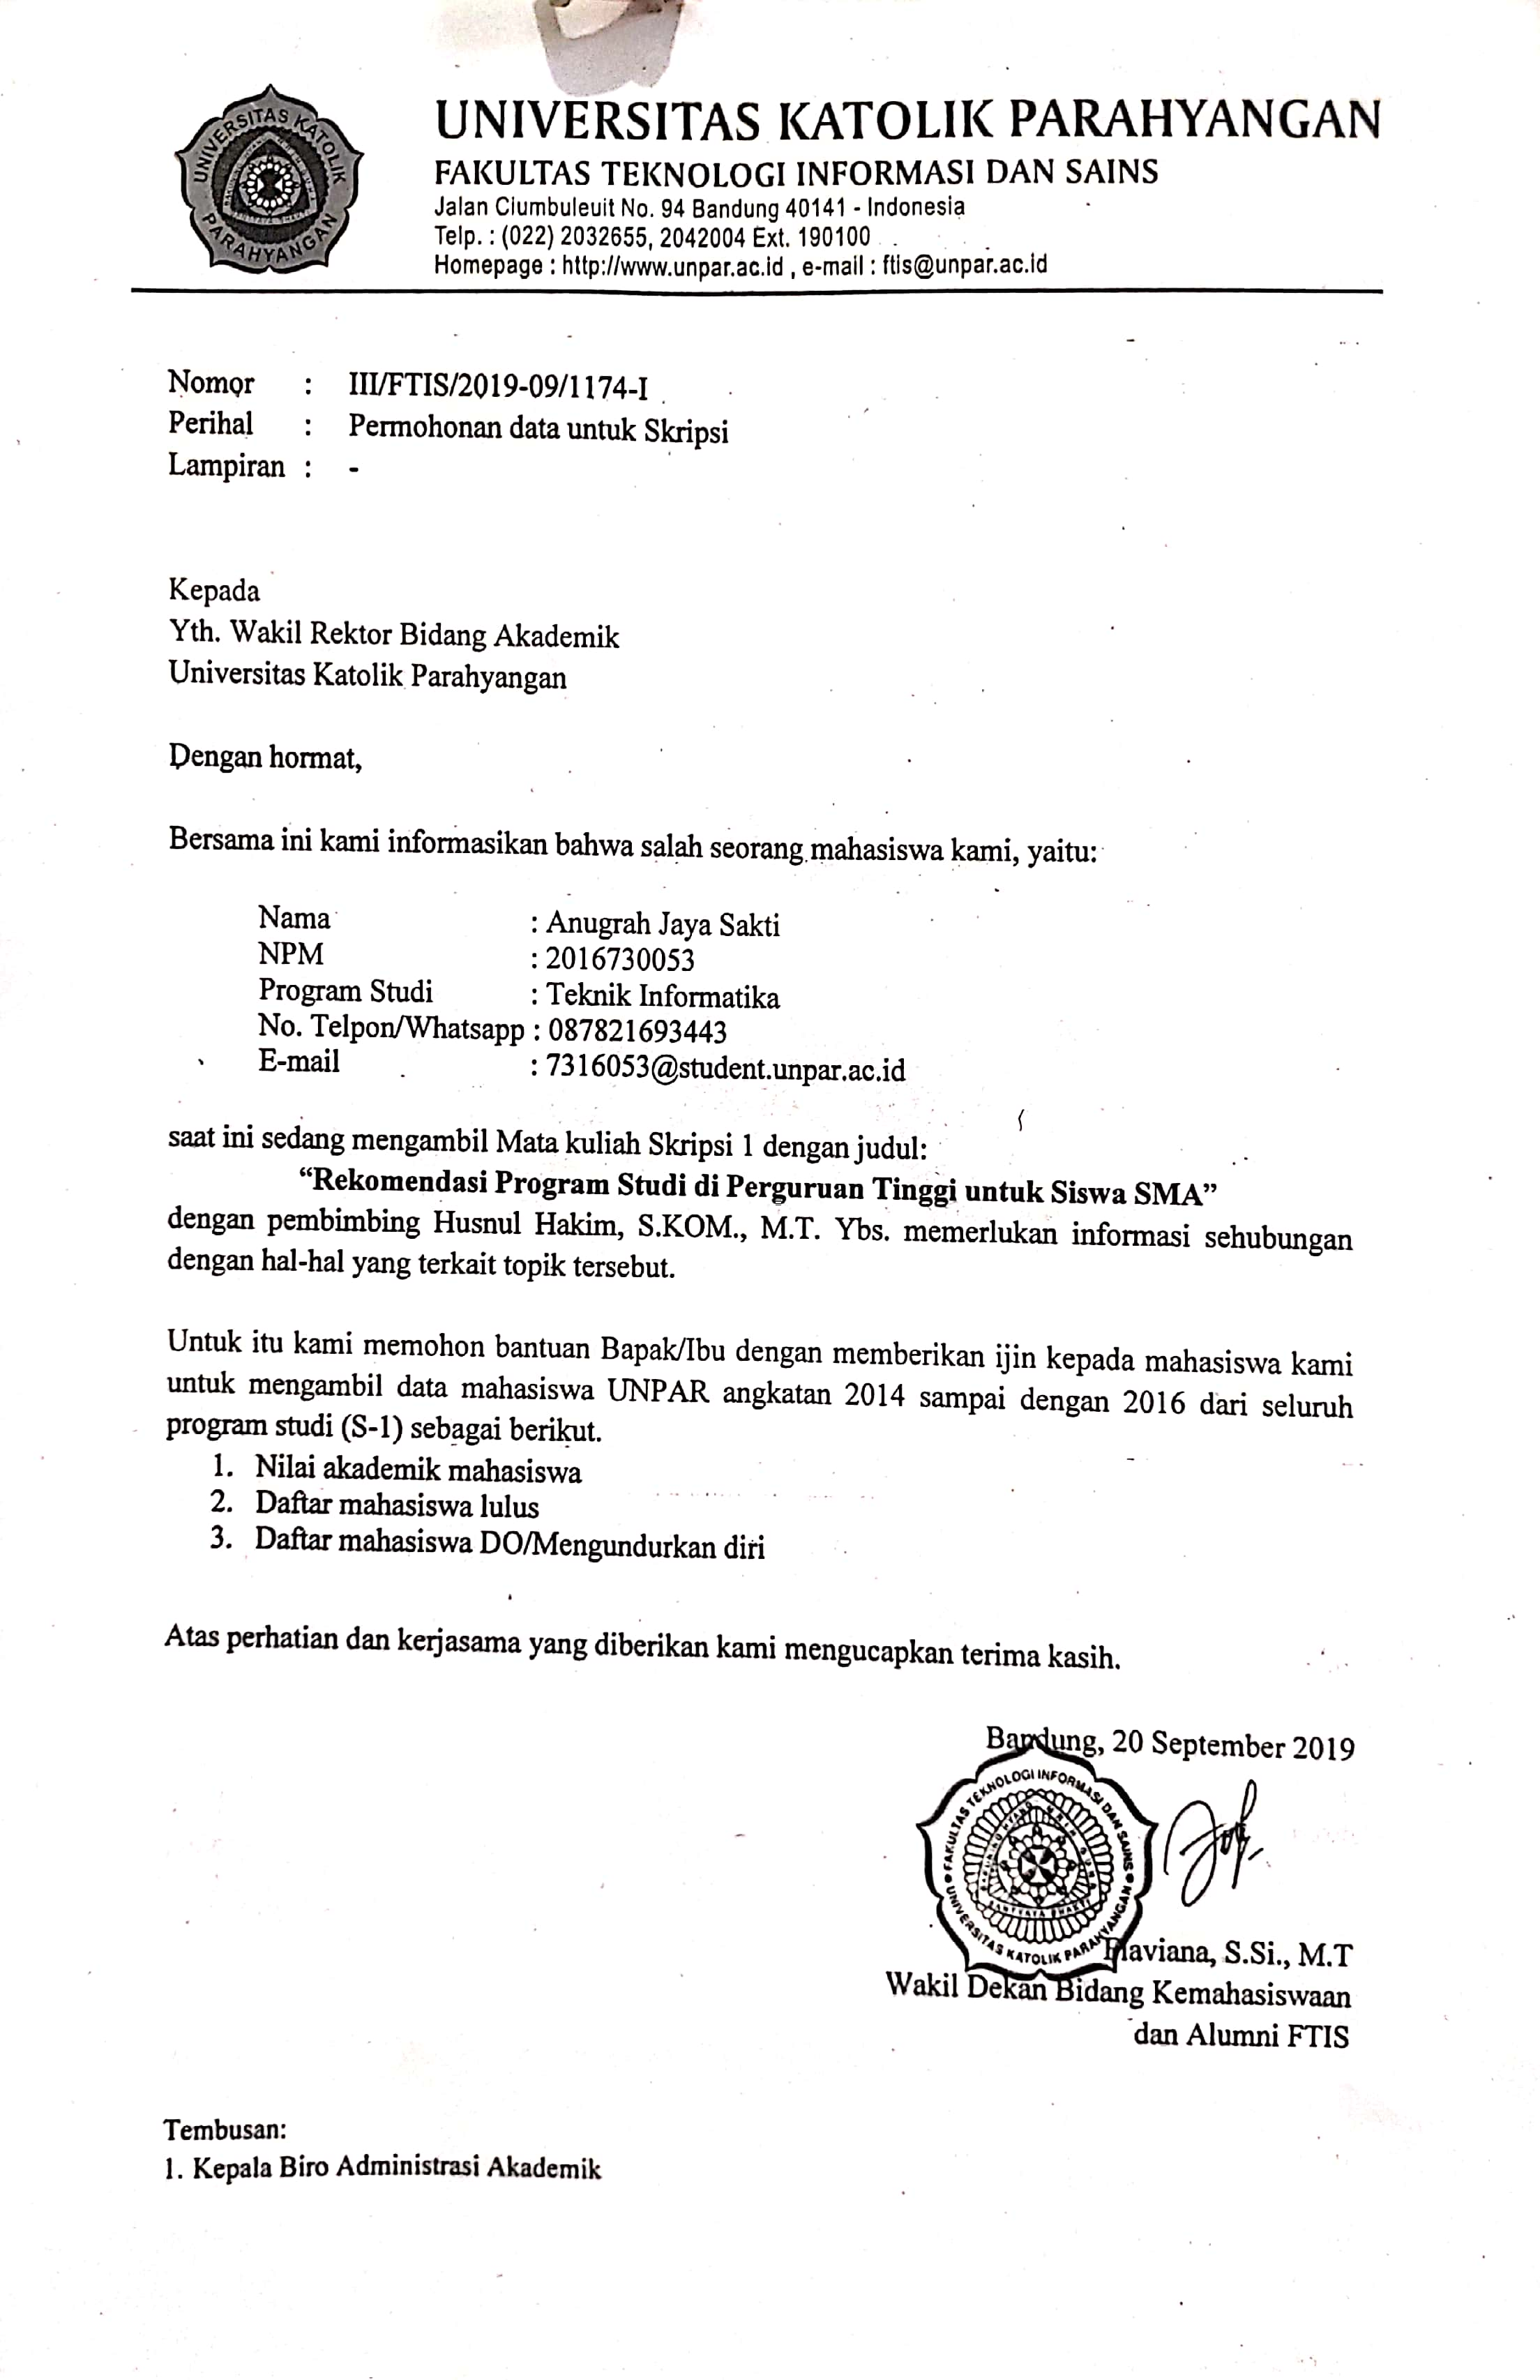
\includegraphics[scale=0.11]{surat}
				\caption{Surat permohonan data}
			\end{figure}
			
			\newpage
			
		\item \textbf{Analisis kebutuhan perangkat lunak}\\
		{\bf Status :} Baru ditambahkan.\\
		{\bf Hasil :} \\
			Kebutuhan perangkat lunak adalah kondisi, kriteria, syarat ataupun kemampuan yang harus dimiliki oleh perangkat lunak untuk memenuhi apa yang diisyaratkan atau diinginkan pemakai. Secara kategoris, ada tiga jenis kebutuhan perangkat lunak, yaitu : 
			\begin{enumerate}
				\item \textit{Functional Requirement}\\
				\textit{Functional Requirement} atau bisa disebut kebutuhan operasional, yaitu kebutuhan yang berkaitan dengan fungsi atau proses transformasi yang harus dapat dikerjakan oleh perangkat lunak. Pada sistem yang akan dibangun harus memiliki kebutuhan fungsional sebagai berikut : Perangkat lunak dapat memberikan rekomendasi item yang relevan dengan pengguna
				
				\item \textit{Interface Requirement}\\
				\textit{Interface Requirement} yang menghubungkan perangkat lunak dengan elemen perangkat keras. Pada sistem yang akan dibangun memiliki kebutuhan antarmuka sebagai berikut : Perangkat untuk masukkan data menggunakan keyboard dan mouse
				
				\item \textit{Performance Requirement}\\
				\textit{Performance Requirement} adalah kebutuhan yang menetapkan karakteristik untuk kerja yang harus dimiliki perangkat lunak, seperti kecepatan, ketepatan, atau frekuensi. Pada sistem yang akan dibangun sebaiknya memiliki \textit{Performance Requirement} sebagai berikut : Akurasi sistem harus lebih besar dari 51\%, karena jika nilai akurasi bisa mencapai minimal 51\% menandakan bahwa hasil prediksi yang sesuai lebih besar dari hasil prediksi yang tidak sesuai berdasarkan dataset yang digunkan untuk pengujian dan pelatihan.
				
			\end{enumerate}
			
			Adapun beberapa batasan sistem yang akan dibangun sebagai berikut :
			\begin{enumerate}
				\item Masukkan berupa nilai bilangan dengan range 0 - 100
				\item Keluaran berupa program studi sesuai dengan jurusan pada saat SMA
				\item Sistem hanya dapat digunakan untuk bagi yang ingin kuliah di UNPAR
			\end{enumerate}
		
		\item \textbf{Menulis sebagian dokumen skripsi.}\\
		{\bf Status :} Ada sejak rencana kerja skripsi.\\
		{\bf Hasil :} \\
		Dokumen skripsi yang sudah di tulis sampai saat ini adalah Bab 1 dan Bab 2.
	\end{enumerate}

\section{Pencapaian Rencana Kerja}
Langkah-langkah kerja yang berhasil diselesaikan dalam Skripsi 1 ini adalah sebagai berikut:
\begin{enumerate}
\item Melakukan studi literatur tentang sistem rekomendasi
\item Mempelajari tentang berbagai program studi dan karateristiknya
\item Mempelajari metode yang dapat digunakan untuk menghitung tingkat kecocokan calon mahasiswa dengan program studi
\item Menganalisis hal-hal yang mempengaruhi kecocokan program studi dengan calon mahasiswa
\item Analisis kebutuhan perangkat lunak
\item Menulis sebagian dokumen skripsi
\end{enumerate}



%\section{Kendala yang Dihadapi}
%TULISKAN BAGIAN INI JIKA DOKUMEN ANDA TIPE A ATAU C
%Kendala - kendala yang dihadapi selama mengerjakan skripsi :
%\begin{itemize}
%	\item Terlalu banyak melakukan prokratinasi
%	\item Terlalu banyak godaan berupa hiburan (game, film, dll)
%	\item Skripsi diambil bersamaan dengan kuliah ASD karena selama 5 semester pertama kuliah tersebut sangat dihindari dan tidak diambil, dan selama 4 semester terakhir kuliah tersebut selalu mendapat nilai E
%	\item Mengalami kesulitan pada saat sudah mulai membuat program komputer karena selama ini selalu dibantu teman
%\end{itemize}

\vspace{1cm}
\centering Bandung, \tanggal\\
\vspace{2cm} \nama \\ 
\vspace{1cm}

Menyetujui, \\
\ifdefstring{\jumpemb}{2}{
\vspace{1.5cm}
\begin{centering} Menyetujui,\\ \end{centering} \vspace{0.75cm}
\begin{minipage}[b]{0.45\linewidth}
% \centering Bandung, \makebox[0.5cm]{\hrulefill}/\makebox[0.5cm]{\hrulefill}/2013 \\
\vspace{2cm} Nama: \pembA \\ Pembimbing Utama
\end{minipage} \hspace{0.5cm}
\begin{minipage}[b]{0.45\linewidth}
% \centering Bandung, \makebox[0.5cm]{\hrulefill}/\makebox[0.5cm]{\hrulefill}/2013\\
\vspace{2cm} Nama: \pembB \\ Pembimbing Pendamping
\end{minipage}
\vspace{0.5cm}
}{
% \centering Bandung, \makebox[0.5cm]{\hrulefill}/\makebox[0.5cm]{\hrulefill}/2013\\
\vspace{2cm} Nama: \pembA \\ Pembimbing Tunggal
}
\end{document}

